\documentclass{standalone}
\usepackage{tikz}
\usetikzlibrary{decorations.pathreplacing}
\usepackage{amsfonts}


\begin{document}
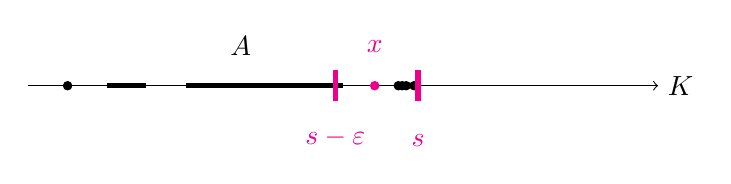
\begin{tikzpicture}
% Draw the real line
  \draw[->] (-4,0) -- (4,0) node[right] {$K$};
  
  % Draw the point 'x' and '0'
   
  \filldraw (-3.5,0) circle (1.5pt); 
 
  \draw[black, line width=2pt] (-3,0) -- (-2.5,0);
    \draw[black, line width=2pt] (-2,0) -- (0,0);


  \filldraw[magenta] (0.4,0) circle (1.5pt);
  \node[magenta, anchor=north] at (0.4,0.7) {$x$}; 
  
  \filldraw (0.7,0) circle (1.5pt);
  \filldraw (0.75,0) circle (1.5pt);
  \filldraw (0.8,0) circle (1.5pt);
  \filldraw (0.9,0) circle (1.5pt);
  
  \node at (-1.3, 0.5) {$A$};
  
  % Draw the brace and label it

  

  \node[magenta, anchor=south] at (-0.1,-0.9) {$s - \varepsilon$}; 
  \draw[line width=2pt, magenta] (-0.1,-0.2) -- (-0.1,0.2);
  
  \node[magenta, anchor=south] at (0.95,-0.9) {$s$}; 
  \draw[line width=2pt, magenta] (0.95,-0.2) -- (0.95,0.2);
  
  
  
  
  
  \end{tikzpicture}
\end{document}